\documentclass{article}
\usepackage{tenor2015}
\usepackage{times}
\usepackage{ifpdf}
\usepackage[english]{babel}
\usepackage{cite}
\usepackage{microtype}

\usepackage[scaled=0.95]{inconsolata}
\usepackage{verbatim}

\usepackage{listings}
\lstset{language=Python,
showspaces=false,
showtabs=false,
breaklines=false,
showstringspaces=false,
breakatwhitespace=false,
escapeinside={(*@}{@*)},
keywordstyle=\bfseries,
basicstyle=\scriptsize\ttfamily
}

\def\papertitle{The design priorities behind Abjad:
Architecting an open-source software system for Formalized Score Control}
\def\firstauthor{Trevor Ba\v{c}a}
\def\secondauthor{Josiah Wolf Oberholtzer}
\def\thirdauthor{Jeffrey Trevi\~{n}o}
\def\fourthauthor{V\'{i}ctor Ad\'{a}n}

\newif\ifpdf
\ifx\pdfoutput\relax
\else
   \ifcase\pdfoutput
      \pdffalse
   \else
      \pdftrue
\fi

\ifpdf % compiling with pdflatex
  \usepackage[pdftex,
    pdftitle={\papertitle},
    pdfauthor={\firstauthor, \secondauthor, \thirdauthor, \fourthauthor},
    bookmarksnumbered, % use section numbers with bookmarks
    pdfstartview=XYZ % start with zoom=100% instead of full screen; 
                     % especially useful if working with a big screen :-)
   ]{hyperref}
  %\pdfcompresslevel=9

  \usepackage[pdftex]{graphicx}
  % declare the path(s) where your graphic files are and their extensions so 
  %you won't have to specify these with every instance of \includegraphics
  \graphicspath{{./figures/}}
  \DeclareGraphicsExtensions{.pdf,.jpeg,.png}

  \usepackage[figure,table]{hypcap}

\else % compiling with latex
  \usepackage[dvips,
    bookmarksnumbered, % use section numbers with bookmarks
    pdfstartview=XYZ % start with zoom=100% instead of full screen
  ]{hyperref}  % hyperrefs are active in the pdf file after conversion
  \usepackage[dvips]{epsfig,graphicx}
  \graphicspath{{./figures/}}
  \DeclareGraphicsExtensions{.eps}
  \usepackage[figure,table]{hypcap}
\fi

\hypersetup{
    colorlinks,
    citecolor=black,
    filecolor=black,
    linkcolor=black,
    urlcolor=black
}

%\title{\papertitle}
\title{The design priorities behind Abjad: \\ 
Architecting an open-source software system \\
for Formalized Score Control}

\fourauthors
  {\firstauthor} {Harvard University \\
    {\tt \href{mailto:trevor.baca@gmail.com}
        {trevor.baca@gmail.com}}}
  {\secondauthor} {Harvard University \\
    {\tt \href{mailto:josiah.oberholtzer@gmail.com}
        {josiah.oberholtzer@gmail.com}}}
  {\thirdauthor} {Carleton College \\
    {\tt \href{mailto:jeffrey.trevino@gmail.com}
        {jeffrey.trevino@gmail.com}}}
  {\fourthauthor} { 
    {\tt \href{mailto:vctradn@gmail.com}
        {vctradn@gmail.com}}}

\begin{document}

\capstartfalse
\maketitle
\capstarttrue

\begin{abstract}
Abjad\footnote{www.projectabjad.org} is an interactive open-source software
system designed to help composers build up complex pieces of music notation in
an iterative and incremental way.  Abjad is implemented in the
Python\footnote{www.python.org} programming language and architected as an
object-oriented collection of packages, classes and functions. Composers can
visualize their work as publication-quality score at all stages of the
compositional process using Abjad's interface to the
LilyPond\footnote{www.lilypond.org} music notation package. Although the first
versions of Abjad were implemented in 1997 and the project website is now
visited thousands of times each month, we have never documented the design
priorities that have guided us as we have built the system. In this paper we
detail some of the most important principles we have followed in our work
architecting Abjad. The priorities we document here arise in answer to
domain-specific questions of music modeling (what are the fundamental elements
of music notation? which elements of music notation should be modeled
hierarchically? which programming constructs are available to help model the
temporal relationships arising between entities in musical score?) as well as
in consideration of the ways in which best practices taken from software
engineering can apply to the development of a music software system like ours
(which programming concepts concerning things like iteration, aggregation and
encapsulation make sense to make available to composers? which existing tools
to test, document and deploy other open-source projects are available to help
develop a music software system like Abjad?). In the sections that follow we
discuss the background and motivations that lead us to ask questions like these
and then elaborate the design priorities we have arrived at in our ongoing work
architecting Abjad.
\end{abstract}

\section{Background \& Motivations} \label{sec:background}

While many environments for both notation and sound production have arisen
within the last twenty years, the following discussion focuses solely on the
production of notation: Abjad enables composers to express both low- and
high-level compositional ideas by extending a widely used programming language
to provide a sufficiently detailed object model of common practice musical
notation. To minimize the restriction of artistic thought's infinite
possibility while maximizing the ability to specify elegantly any arbitrary
symbolic relationship, Abjad does this without prescribing explicit or implicit
models of music or composition: Abjad defines composition narrowly as the act
of creating a document via the encoded aggregation of notational symbols.

\subsection{Generative Task as an Analytic Framework}

Software production exists as an organizationally designed feedback loop
between production values and implementation \cite{Derniame:1999fk}, and it is
possible to understand a system by understanding the purpose for which it was
initially designed, the system's \emph{generative task(s)}. In the analysis of
systems created for use by artists, this priority yields a dilemma instantly,
as analyses that explain a system's affordances with reference to intended
purpose must contend with the creative use of technology by artists: a system's
intended uses might have little or nothing in common with the way in which the
artist finally uses the technology. For this reason, the notion of generative
task is best understood as an explanation for a system's affordances, with the
caveat that a user can nonetheless work against those affordances to use the
system in novel ways. Generative tasks --- informed by the cultural milieu of
software development, economic constraints of software production, and the
aesthetic proclivities of artists participating in development processes ---
constrain software features to enable a limited subset of possible
representations and user interactions.

While composers working traditionally may allow intuition to substitute for
formally defined principles, a computer demands the composer to think formally
about music \cite{Xenakis:1992rq}. Keeping in mind generative task as an
analytical framework, it is broadly useful to bifurcate an automated notation
system's development into the modeling of music and composition, on the one
hand, and the modeling of musical notation, on the other. All systems model
both, to greater or lesser degrees, often engaging in the ambiguous or implicit
modeling of music and composition while focusing more ostensibly on a model of
notation, or focusing on the abstract modeling of music without a considered
link to a model of notation. Due to the intimate link between notation and
musical ideas, it is impossible for a system that models notation to avoid at
least implicitly modeling musical and compositional ideas, and a computational
model of music and composition is an inevitable component of every automated
notation system, even when it exists as an unspoken set of technological
constraints. Generative task explains a given system's balance between
computational models of music/composition and notation by assuming a link
between intended use and system development.

\subsection{Computational Models of Notation}

Many systems implement detailed models of music explicitly or implicitly, but
few of these implement detailed models of notation.\footnote{Computational
models of music might entail the representation of higher-level musical
entities apparent in the acts of listening and analysis but absent in the
symbols of notation themselves, as determined to be creatively exigent.
Programming researchers and musical artists have modeled many such
extrasymbolic musical entities, such as large-scale form and transition
\cite{polansky1991morphological}, \cite{uno1994temporal},
\cite{dobrian1995algorithmic}, \cite{abrams1999higher}, \cite{Yoo1983}, texture
\cite{Horenstein:2004kx}, contrapuntal relationships \cite{Boenn:2009oq},
\cite{Acevedo2005}, \cite{Anders:2011kl}, \cite{Balser:1990tg},
\cite{Jones:2000hc}, \cite{uno1994temporal}, \cite{Bell:1995ij},
\cite{farbood2001analysis}, \cite{Cope:2002fv}, \cite{Laurson:2005dz},
\cite{Polansky:2011fu}, \cite{Ebcioglu:1980kl}, harmonic tension and resolution
\cite{Melo2003}, \cite{Wiggins1999}, \cite{Foster:1995qa}, melody
\cite{Hornel:1993mi}, \cite{Smith:1992pi}, meter \cite{Hamanaka:2005ff}, rhythm
\cite{Nauert2007}, \cite{Degazio:1996lh}, \cite{Collins:2003bs}, timbre
\cite{Xenakis:1991fu}, \cite{Creasey:1996ye}, \cite{Osaka2004}, temperament
\cite{Seymour:2007qo}, \cite{Graf:2006il}, and ornamentation
\cite{Ariza:2003zt}, \cite{Chico-Topfer:1998jl}. This work overlaps fruitfully
with analysis tasks, and models of listening and cognition can enable novel
methods of high-level musical structures and transformations, like dramatic
direction, tension, and transition between sections \cite[108]{Collins2009}.} A
system that affords a detailed model of music/composition without linking to a
sufficiently detailed model of musical notation does not afford automated
notation --- sufficiency, however, depends heavily on generative task. For
example, if a composer requires an automated notation system to render complex
rhythmic ideas that depend typographically on nested tuplets, a system that
produces a notation only via a combination of MIDI and quantization must reduce
rhythms to a non-hierarchical stream of event times, eliminating the temporally
divisive approach of tuplet notation. For many rhythmic applications, though,
MIDI suffices. 

Many automated notation systems exist to model musical notation and the act of
typographical layout without explicitly affording the computational modeling of
music or composition \cite{Smith:1972mw}, \cite{Nienhuys:2003ve},
\cite{Hoos:1998bd}, \cite{hamel1noteability}; many of these systems strongly
imply a model of music, such as Gr\'{e}goire for Gregorian chant, Django for
guitar tablature, and GOODFEEL for Braille notation \cite{2006}, while
feature-rich systems (often oriented toward classical composers) such as
Finale, Sibelius, SCORE, Igor, Berlioz, and Nightingale, present themselves as
relatively more genre-agnostic software tools. Such a system might go so far as
to enable a text-based object-oriented model of notation that automates some
aspect of an otherwise point-and-click interface, as in the case of Sibelius's
ManuScript scripting language \cite{Technology:qc}. 

Many models of musical notation have been designed created for purposes of
corpus-based computational musicology. Formats such as Music21, DARM, SMDL,
HumDrum, and MuseData model notation with the generative task of searching
through a large amount of data \cite{Selfridge-Field:1997ud}. Commercial
notation software developers attempted to establish a data interchange standard
for optical score recognition (NIFF) \cite{niff1995niff}; since its release in
2004, MusicXML has become a valid interchange format for over 160 applications
and maintains a relatively application-agnostic status, as it was designed with
the generative task of acting as an interchange format between variously tasked
systems \cite{Good:2001if}. (are Igor and Berlioz commercial?)

Notation representations that underly many of these GUI-based systems often go
undescribed as computer representations of notation, in favor of discussions
about human-computer interaction. For example, Barker and Cantor developed an
early model of music notation that underlies a four-oscilloscope GUI and
describe their work entirely in terms of user interaction
\cite{cantor1971computer}; likewise, discussions of modern commercial notation
systems remain similarly oriented, without much awareness or criticism of the
underlying computational models of notation. This results in insufficiently
detailed models of notation; systems, for example, that provide models only of
mensural notation and enable nonmensural notations only as modified
instantiations of notations based on measures.

\subsection{The Development of Hierarchical Object Models of Notation}

Many early models of musical notation were not hierarchical, and Lejaran
Hiller, in reflecting on decades of automated notation work, identifies the
lack of hierarchical organization as a limitation of early work --- although
Nick Collins points out that even Hiller's program PHRASE addresses the
hierarchical organization of a score up to the level of a phrase, without
moving beyond this mid-level musical structure to concerns of large-scale form
\cite[108]{Collins2009}. 

There were several object-oriented music environments by 1990
\cite[139]{Polansky:1990fk}, most created in or inspired by the newly popular
Smalltalk-80 programming language; while they facilitated the hierarchical
modeling of musical abstractions, they omitted or radically simplified the
hierarchical nature of common notation. For example, Glen Krasner (Xerox
Systems Science Laboratory) created Machine Tongues VIII, a music system that
created an object-oriented model of the score/orchestra distinction inherited
from Max Mathews' Music N languages, with a simple linear model of ``partOn''
and ``partOff'' command sequences \cite{Krasner:1991uq}, omitting hierarchical
organization entirely when the system produced notational output; although
subsequent Machine Tongues systems introduced some hierarchical organization
via ``note'' objects that inhabited ``event lists,'' systems did not attempt to
model the hierarchical detail of all a traditional score's elements. Like
Hiller's PHRASE program, Andreas Mahling's CompAss system organized events
hierarchically up to the mid-level ``phrase'' level of musical structure
\cite{Mahling:1991qf}. These systems extend Smalltalk-80 with interfaces to the
MIDI communications protocol: as extensions of Smalltalk, they enabled the user
to arbitrarily extend the system with new objects, creating a detailed and
hierarchical model of music, usually flattened into a list of noteOn and
noteOff commands to be notated or played back via MIDI interface. 

By 1989, Glendon Diener's Nutation system (written in Objective C for the NeXT
computer) modeled both musical and notational structure hierarchically through
the use of directed graphs \cite{Diener:1991zr}, \cite{Diener:1991ly},
\cite{Diener:1989ve}.

last section: system motivations

Linking our design priorities with those of previous systems by describing
perceived deficiencies: evaluative priorities for previous systems: sufficiency
instead of comprehensiveness, potentially evaluated by sonic result rather than
notation, addressability (in HMSL and JMSL). Reintroduce generative task: late
50s through 80s were motivated locally by generative tasks of specific projects
until IRCAM's Patchwork approached a generative task of broadly enabling
composers; sufficiency determined by comprehensive task.

\section{Extension, not reinvention} \label{sec:extension}

Abjad is not a programming langauge. Abjad instead extends the Python
programming language. Our insistence on this principle of extension --- of
adding functionality to an existing programming language rather than inventing
yet another domain-specific language --- originates in the belief that there is
no real benefit to be had in reestablishing the ways variables are created,
references are handled, loops are structured or any of the other fundamentals
of programming. We have instead architected Abjad in the form of a Python
package designed to be used the same way as the thousands of other packages
that equip Python with new functionality.\footnote{See the Python Package Index
for functionality to extend the language for purposes as diverse as creative
writing and aeronautical engineering. The Python Package Index contains 54,306
packages at the time or writing and is available at \textit{pypi.python.org}.}
In designing Abjad as an extension to a widely used language we make relevant
both the hundreds of already-available print and Web resources that detail
Python and its features as well as the global community of developers working
in the language. Both benefits we hope to ease composers' transition to
programming and make working with Abjad a familiar task that conforms to
programming best practices: there will probably by necessity always
be more programmers than composers in the world and it makes sense for our work
as composers to benefit from the patterns already understood elsewhere in the
culture.

Though we continue to find Python an excellent programming
language,\footnote{Aspects of Python we find particularly helpful include the
availability of lists, dictionaries and sets as built-in types; the interface
provided for string and Unicode objects; the unified approach to encapsulation
provided by Python's understanding of namespaces; and the extensive
functionality provided in the standard library.} our decision to implement
Abjad in Python does not arise from the specifics of the language but from the
large community of users the language supports and the fact that Python is open
source. The history of music software systems is littered with projects that
fell into disuse. Music software systems except for the large commercial
notation packages will probably always be the niche efforts of specialists and
our experience architecting Abjad leads us to think about the future in such a
way that we give ourselves all the advantages of expansiveness that are
possible: picking an existing language that makes learning preliminaries
easier and makes the continued development of the system as open as possible to
as many different collaborators as possible.

\section{Pervasive illustration} \label{sec:illustration}

We believe it is important for composers to be able to illustrate the objects
they work with as they compose. Abjad reflects this priority in its
\emph{illustration protocol}.\footnote{Python describes common informal
interfaces to working with objects as \emph{protocols}. Important protocols
include the \emph{iterator protocol} for iterating over the contents of a
container-like object, the \emph{sequence protocol} for getting items and
length from a container-like object and the \emph{mutable container protocol}
for mutating the contents of a container-like object.} Abjad's illustration
protocol conventionalizes the way developers equip Abjad classes with
illustration output and the way composers access illustration output during
composition. The composer-facing part of the protocol is implemented in Abjad's
top-level \texttt{show()} function, which provides composers a unified way to
illustrate any object in the system. The developer-facing part of Abjad's
illustration protocol is evidenced in the collection of
\texttt{\_\_illustrate\_\_()} methods that define how classes throughout the
system are to illustrate when passed to \texttt{show()}.\footnote{Abjad's
pairing of a single \texttt{show()} function with \texttt{\_\_illustrate\_\_()}
methods defined as needed parallels the way Python's \texttt{len()} function
works with \texttt{\_\_len\_\_()} methods defined on custom classes.} Under the
most common pattern, Abjad transforms an object into LilyPond input code and
then calls LilyPond to render the resultant input as a PDF. In all cases the
composer's interface to the illustration logic implemented on a  class is
provided by \texttt{show()}, as in the examples in this
article.\footnote{Abjad's illustration protocol decouples illustration logic
from the other functions of a class. An important consequence of this is that
developers can illustrate classes with LaTeX or GraphViz or any collection of
applications, whether or not LilyPond is included in the tool chain. We find
LilyPond superior for a formalized score control system like Abjad for many
reasons, ranging from LilyPond's powerful model of rhythmic timekeeping to the
high quality of LilyPond output. But should the need arise to replace LilyPond
with a different typesetting engine, the composer-facing  interface provided by
\texttt{show()} will remain the same. The priority is that composers be able to
illustrate compositional objects. LilyPond simply happens to be the best
resource available to achieve our goals.} 

\section{Bottom-up construction} \label{sec:bottom-up}

We believe composers should be able to build scores from the bottom up. Abjad
never obscures the individual notational elements of the compositional process.
Combining score components piece by piece into ever-larger aggregates gives
composers fine-grained control over their compositional structures. Such
control guarantees a high degree of compositional-process agnosticism on
Abjad's part, and affords composers a solid framework on top of which they can
design and implement their own personal approaches to composition.

%Abjad assumes that symbols on the page --- notational primitives --- are the
%elements of composition. The act of composition then revolves around the
%iterative aggregation of these elements into arbitrarily complex score objects.

\subsection{Components, spanners and indicators}

Abjad models score in terms of \emph{components}, \emph{spanners} and
\emph{indicators}. These families of objects represent all of the notational
primitives in Abjad. Score components include \emph{leaves}\footnote{Abjad
borrows the term \emph{leaf} from graph theory.} --- notes, chords and rests
--- and \emph{containers} --- tuplets, measures, voices, staves, staff groups
and scores and so forth. Components are arranged hierarchically into a tree by
nesting score components inside containers. Child components receive a
reference to their sole parent container, and parent containers maintain
references to their children. Spanners model musical constructs such as beams,
slurs and glissandi which \emph{span} across score components in a single
\emph{logical voice}, allowing for the introduction of cyclicity into the
acyclic component graph by spanning across components in different parentages.
Indicators model objects attached to a single component, including
articulations, time signatures, tempi, textural indications and dynamics.
Indicators can have \emph{scope} making them \emph{effective} for all other
components in that scope following the component to which that indicator is
attached until another indicator of the same type appears. Indicator scoping
models how all notes in a voice can be \emph{forte} until a \emph{piano}
indication appears. We have generalized this behavior, allowing composers to
annotate score structures by attaching arbitrary non-notating objects like
dictionaries or custom classes to any component.

\subsection{Iterative aggregation}

We believe that is is important for composers to be able to construct scores
though iterative aggregation. Any score modelable by Abjad, no matter how
complex, can be constructed by nesting progressively more and more score
components inside one another, and by attaching spanners and indicators onto
the increasingly complex notational aggregate. Abjad affords score component
aggregation via Python's \emph{mutable sequence} protocol, a collection of
instance methods which allow score components to be appended, extended or
inserted into other container-like score components as though they were lists.

\begin{lstlisting}
>>> outer_tuplet_one = Tuplet((2, 3), "d''16 ef'8.")
>>> inner_tuplet = Tuplet((4, 5), "cs''16 e'16 d'2")
>>> outer_tuplet_one.append(inner_tuplet)
>>> outer_tuplet_two = Tuplet((4, 5))
>>> outer_tuplet_two.extend("d'8 r16 b'16 as'16")
>>> tuplets = [outer_tuplet_one, outer_tuplet_two]
>>> upper_staff = Staff(tuplets, name='Upper Staff')
\end{lstlisting}


\begin{lstlisting}
>>> note_one = Note(10, (7, 32))
>>> upper_staff.append(note_one)
>>> note_two = Note(NamedPitch("fs'"), Duration(1, 32))
>>> upper_staff.append(note_two)
\end{lstlisting}


\begin{lstlisting}
>>> lower_staff = Staff(name='Lower Staff')
>>> lower_staff.extend("c8 r8 b8 r8 gf8 r4 cs8")
>>> staff_group = StaffGroup()
>>> staff_group.extend([upper_staff, lower_staff])
>>> score = Score([staff_group])
>>> show(score)
\end{lstlisting}

\noindent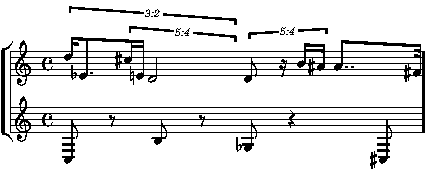
\includegraphics[scale=1.0]{images/abjad-1.pdf}


Composers can attach spanners (such as ties and slurs) to score components via
Abjad's top-level \texttt{attach()} function.

\begin{lstlisting}
>>> upper_leaves = upper_staff.select_leaves()
>>> lower_leaves = lower_staff.select_leaves()
>>> attach(Tie(), upper_leaves[4:6])
>>> attach(Tie(), upper_leaves[-3:-1])
>>> attach(Slur(), upper_leaves[:2])
>>> attach(Slur(), upper_leaves[2:6])
>>> attach(Slur(), upper_leaves[7:])
\end{lstlisting}


Composers can also attach indicators (such as articulations and clefs) to
individual score components with \texttt{attach()}.

\begin{lstlisting}
>>> attach(Articulation('accent'), upper_leaves[0])
>>> attach(Articulation('accent'), upper_leaves[2])
>>> attach(Articulation('accent'), upper_leaves[7])
>>> attach(Clef('bass'), lower_leaves[0])
>>> show(score)
\end{lstlisting}

\noindent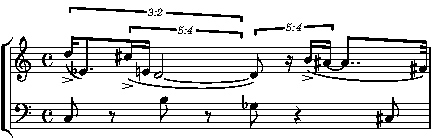
\includegraphics[scale=1.0]{images/abjad-2.pdf}


\subsection{Input flexibility}

We believe that there should be multiple ways of instantiating compositional
elements. Input flexibility affords composers the ability to create
compositional objects in whatever way closest aligns with their conception of
music and their specific task at hand \cite{Kay:1996vn}. Abjad's score components
can be created in a variety of ways. Leaves (such as notes) can be instantiated
parametrically by specifying pitch and rhythm information numerically. Leaves
can also be created via explicit \texttt{Pitch} and \texttt{Duration} objects.
Containers (such as tuplets and measures) can be instantiated parametrically by
specifying explicit lists of components to be inserted as children. Abjad also
allows many score objects to be created via strings parseable in one of the
various micro-languages we have implemented. Score components created via
string input can be potentially much more complex than those created
parametrically because Abjad's microlanguage parsers have the ability to attach
spanners and indicators to the created components or their children, if they
are containers. Parametric instantiation affords composers powerful procedural
control over score structure while string instantiation allows for brevity and
expressiveness. The score construction example above demonstrates both
techniques. 

\section{Top-down construction} \label{sec:top-down}

With experience, use of the system migrates from bottom-up to top-down. We
realize that composers probably don't find it interesting to make a single
note, but can be deeply engaged by the process of creating intermediate and
high-level objects like phrases or complete segments of music. Abstraction,
encapsulation and re-use of generative processes is what comes closest to the
work of beginning to implement one's own system of composition.

\subsection{Factory functions, factory classes}

Abjad provides a variety of factories for quickly and flexibly creating
arbitrarily large amounts of notation. These range from simple leaf-generating
functions like \texttt{scoretools.make\_notes()}, which combine sequences of
pitches and rhythms isorhythmically to generate selections of notes and rests,
to more complexly-configured \emph{maker} classes for creating nuanced rhythmic
patterns or entire scores.

\begin{lstlisting}
>>> notes = scoretools.make_notes([0, 1, 4, 7], [(1, 4)],)
>>> staff = Staff(notes)
>>> show(staff)
\end{lstlisting}

\noindent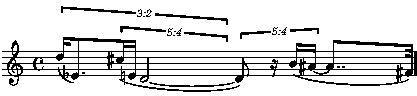
\includegraphics[scale=1.0]{images/abjad-3.pdf}


Abjad's \emph{rhythm makers} are factory classes which, once configured, can be
called like functions to procedurally inscribe rhythms into a series of
\emph{divisions}. The \texttt{NoteRhythmMaker} fills in divisions with notes,
tied as necessary, to equal the duration of those divisions.

\begin{lstlisting}
>>> divisions = [(3, 8), (5, 16), (1, 4), (5, 16)]
>>> rhythm_maker = rhythmmakertools.NoteRhythmMaker()
>>> show(rhythm_maker, divisions=divisions)
\end{lstlisting}

\noindent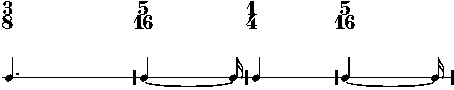
\includegraphics[scale=1.0]{images/abjad-4.pdf}


Other rhythm makers, such as Abjad's \texttt{TaleaRhythmMaker}, can create even
more complex rhythmic output, integrating configurable patterns of durations,
tupletting and silences.

\begin{lstlisting}
>>> rhythm_maker = rhythmmakertools.TaleaRhythmMaker(
...     burnish_specifier=rhythmmakertools.BurnishSpecifier(
...         left_classes=(Rest, Note),
...         left_counts=(1,),
...         ),
...     extra_counts_per_division=(0, 1, 1),
...     talea=rhythmmakertools.Talea(
...         counts=(1, 2, 3),
...         denominator=16,
...         ),
...     tie_specifier=rhythmmakertools.TieSpecifier(
...         tie_across_divisions=True,
...         ),
...     )
>>> show(rhythm_maker, divisions=divisions)
\end{lstlisting}

\noindent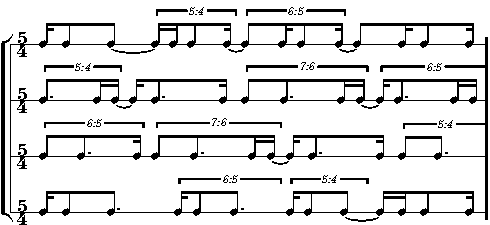
\includegraphics[scale=1.0]{images/abjad-5.pdf}


Once instantiated, rhythm makers can be used over and over again with different
input, a pattern used pervasively in Abjad: maker classes as object-oriented
partially-evaluated functions. As generating duration sequences is generally
less difficult than creating complete tupletted, beamed and tied rhythmic score
artifacts, rhythm makers allow composers to focus on the process of building
rhythm structures as a compositional material in-and-of itself. Because rhythm
makers are classes, they can be subclassed and extended in order to modify
their behavior. Because they are objects, they can be passed as parameters to
configure even more expansive aggregate makers.

\emph{Score templates} are another common factory pattern in Abjad,
encapsulating the work of building the skeletons of complete scores, including
voices, staves, staff groups, clefs and other indications pertinent to the
intended instrumentation or typography. We can combine rhythm and score makers
with score iteration, as well as some simple bottom-up construction, to
generate complete score aggregates expressively.

\begin{lstlisting}
>>> template = templatetools.GroupedStavesScoreTemplate(4)
>>> quartet_score = template()
>>> iterator = iterate(quartet_score).by_class(Voice)
>>> for index, voice in enumerate(iterator):
...     divisions = sequencetools.rotate_sequence(
...         divisions, -1)
...     selections = rhythm_maker(divisions, seeds=-index)
...     measure = Measure((5, 4), selections)
...     voice.append(measure)
... 
>>> show(quartet_score)
\end{lstlisting}

\noindent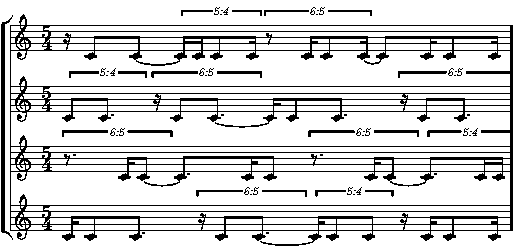
\includegraphics[scale=1.0]{images/abjad-6.pdf}


\subsection{Top-down extensibility}

We believe that there are more ways to generate notation than we can conceive
of. While Abjad has implemented many notational factories, we do not think
these are sufficient for any one artist's process and have therefore
architected the project in such a way as to encourage extension by composers
interacting with the system in the spirit of compositional agnosticism.

%By providing core functionality oriented toward the elements of standard
%notation, Abjad strives to remain as agnostic as possible to various
%composition techniques. 

\section{Selection flexibility} \label{sec:selections}

we think it's important for composers to be able to select arbitrary
collections of score objects. this is important for a couple of reasons. first,
so that composers can map operations to the entirety of such a selection at one
time. second, there's some type of conceptual benefit to be had in named
selections; the point is that every selection is an ad hoc intermediate
structure created in the midst of the score. we also think it's important to
afford composers the ability to reference score objects in whatever ways are
most natural for a given task. sometimes the most natural mode of reference is
numeric, sometimes by name or sometimes by music-specific criteria such as the
relative times at which different objects appear in the score. examples follow.
we provide concrete object models of vertical relationships in the score.

selecting one object: by number, by time relation, by name.

selecting many things: by slicing, by select\_leaves(), by iteration.

[TREVOR]

%Abjad allows the numeric addressing of all score components. Abjad score
%components are zero-indexed from the start of the container which holds them:
%the statement \texttt{staff[0]} addresses the first component contained in
%\texttt{staff} while the statement \texttt{staff[1]} addresses the component
%after that, and so on. Negative indices address components from the end of the
%container which holds them. Python's slice notation may be used to retrieve an
%arbitrary number of contiguous components at one time. As an example of the
%latter, the statement \texttt{staff[15:25]} selects the ten components in
%\texttt{staff} between indices 15 and 25. The conventions of Abjad's numeric
%addressing regime follow those of Python's list and tuple interface exactly. 

Consider the two-staff score created earlier. The upper staff can be selected
by indexing the first child of the first child of the score, i.e. the first
staff in the staff group which is the first child of the score itself.

\begin{lstlisting}
>>> upper_staff = score[0][0]
>>> show(upper_staff)
\end{lstlisting}

\noindent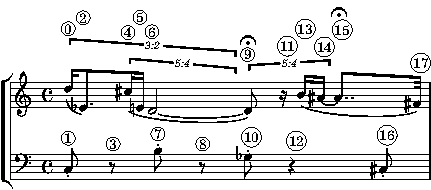
\includegraphics[scale=1.0]{images/abjad-7.pdf}


Because both staves were given explicit names, they can also be selected by
those names, regardless of their depth in the score hierarchy.

\begin{lstlisting}
>>> lower_staff = score['Lower Staff']
>>> show(lower_staff)
\end{lstlisting}

\noindent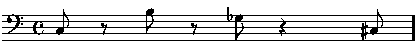
\includegraphics[scale=1.0]{images/abjad-8.pdf}


A score container's leaves --- the notes, chords and rests at the bottom of the
score hierarchy which cannot, by definition, contain any other score component
--- can be selected by that container's \texttt{select\_leaves()} method.

\begin{lstlisting}
>>> for leaf in lower_staff.select_leaves():
...     print(repr(leaf))
... 
Note('c8')
Rest('r8')
Note('b8')
Rest('r8')
Note('gf8')
Rest('r4')
Note('cs8')
\end{lstlisting}


Composers can select components via Abjad's powerful top-level
\texttt{iterate()} function, which exposes the score iteration interface as
implemented in our \texttt{IterationAgent}. The iteration interface affords a
wide variety of selection criteria, such as class filters, logical tie
selection and time-wise score traversal.

\begin{lstlisting}
>>> for note in iterate(lower_staff).by_class(Note):
...     attach(Articulation('staccato'), note)
... 
>>> show(score)
\end{lstlisting}

\noindent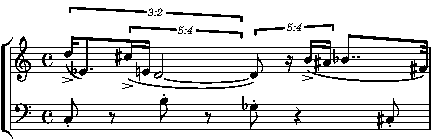
\includegraphics[scale=1.0]{images/abjad-9.pdf}


\begin{lstlisting}
>>> iterator = iterate(score).by_logical_tie(
...     nontrivial=True, pitched=True)
>>> for logical_tie in iterator:
...     attach(Fermata(), logical_tie.tail)
... 
>>> show(score)
\end{lstlisting}

\noindent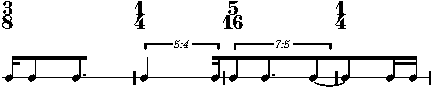
\includegraphics[scale=1.0]{images/abjad-10.pdf}


\begin{lstlisting}
>>> iterator = iterate(score).by_timeline()
>>> for index, component in enumerate(iterator):
...     markup = Markup(index, Up).circle()
...     attach(markup, component)
... 
>>> show(score)
\end{lstlisting}

\noindent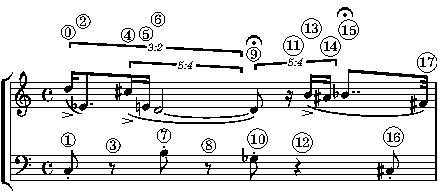
\includegraphics[scale=1.0]{images/abjad-11.pdf}


\section{Configuration} \label{sec:configuration}

%We think it's important for composers to be able to define an operation one
%time and be able to apply the operation to arbitrarily many objects in the
%score at once.

%of the many ways abjad provides of doing this, the most important (and most
%general) is iteration.

%examples follow.

%iteration can be glossed as "define-once, apply-many".

%"configuration reuse".

%we think it's important for composers to be able to configure objects a single
%time, and then resuse the configuration as many times as necessary while
%composing.

%we also think it's important to configure complex objects all at once.

%"templating".

%we think it's important for composers to be able to template all objects in
%the system, especially the hugely complex objects.

%selectors.

\subsection{Nested configuration}

Text here.

\subsection{Templating}

As demonstrated earlier, Abjad's \emph{rhythm makers} are highly-configurable
factory classes for generating rhythmic patterns. Many of their initialization
keywords expect \emph{specifiers} --- object-oriented bundles of related
parameters --- which can make their configurations potentially deeply nested.

\begin{lstlisting}
>>> rhythm_maker = rhythmmakertools.TaleaRhythmMaker(
...     talea=rhythmmakertools.Talea(
...         counts=(1, 2, 3),
...         denominator=16,
...         ),
...     )
>>> print(format(rhythm_maker))
rhythmmakertools.TaleaRhythmMaker(
    talea=rhythmmakertools.Talea(
        counts=(1, 2, 3),
        denominator=16,
        ),
    )
\end{lstlisting}


\begin{lstlisting}
>>> divisions = [(3, 8), (1, 4), (5, 16), (1, 4)]
>>> show(rhythm_maker, divisions=divisions)
\end{lstlisting}

\noindent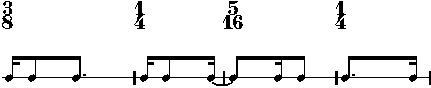
\includegraphics[scale=1.0]{images/abjad-12.pdf}


Nested configuration via parameter grouping with specifiers provides
considerable conceptual clarity, but is also potentially labor-intensive. Abjad
mitigates the work of complex configuration by affording composers with
powerful templating tools. New objects can be created from old ones, optionally
replacing any initialization parameter in the templated object at any depth via
the top-level \texttt{new()} function. Notice how the new rhythm maker below
has both altered its talea counts and added a new initialization keyword.

\begin{lstlisting}
>>> new_rhythm_maker = new(rhythm_maker,
...     extra_counts_per_division=(0, 1),
...     talea__counts=(1, 2, 3, 4),
...     )
>>> print(format(new_rhythm_maker))
rhythmmakertools.TaleaRhythmMaker(
    talea=rhythmmakertools.Talea(
        counts=(1, 2, 3, 4),
        denominator=16,
        ),
    extra_counts_per_division=(0, 1),
    )
\end{lstlisting}


\begin{lstlisting}
>>> show(new_rhythm_maker, divisions=divisions)
\end{lstlisting}

\noindent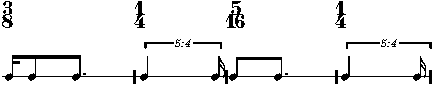
\includegraphics[scale=1.0]{images/abjad-13.pdf}


Repeating the templating process creates new and different yet still related
objects, allowing composers to easily play with variation at the level of
procedure.

\begin{lstlisting}
>>> new_new_rhythm_maker = new(new_rhythm_maker,
...     extra_counts_per_division=(0, 1, 2),
...     beam_specifier=rhythmmakertools.BeamSpecifier(
...         beam_divisions_together=True,
...         ),
...     )
>>> print(format(new_new_rhythm_maker))
rhythmmakertools.TaleaRhythmMaker(
    talea=rhythmmakertools.Talea(
        counts=(1, 2, 3, 4),
        denominator=16,
        ),
    extra_counts_per_division=(0, 1, 2),
    beam_specifier=rhythmmakertools.BeamSpecifier(
        beam_each_division=True,
        beam_divisions_together=True,
        ),
    )
\end{lstlisting}


\begin{lstlisting}
>>> show(new_new_rhythm_maker, divisions=divisions)
\end{lstlisting}

\noindent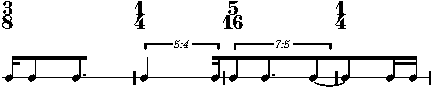
\includegraphics[scale=1.0]{images/abjad-14.pdf}


\section{Encapsulation} \label{sec:encapsulation}

We want everything to be encapsulated as much as possible. what this comes out
to mean is the system is overwhelming object-oriented (in the proper uses of
the term) and that all parts of the system (whether object-oriented or not) are
structured in such a way as to provide a single interface named according to a
uniform set of naming conventions. [TREVOR]

\section{Open-source best practices} \label{sec:open-source}

During the architecting of Abjad we have tried to adhere to as many of the programming best practices developed by the open-source community as possible.

\subsection{Extensibility}

As an open-source project, composers and researchers can contribute changes via
git pull requests. A process of continuous integration and online version
control simplifies this contribution process. 

\subsection{Embeddability}

Abjad is an importable Python library. It can be used in whole or in part as a
component of any Python-compatible system. Abjad has few Python package
dependencies and is not bound to any specific user application or graphic user
interface. These qualities make Abjad an ideal project ideal for embedding in
other software systems.

For example, Abjad supports IPython
Notebook\footnote{http://ipython.org/notebook.html}, a web-based interactive
computational environment combining code execution, text, mathematics, plots
and rich media into a single document. Notational output from Abjad can be
transparently captured and embedded directly into an IPython Notebook which has
loaded Abjad's IPython Notebook extension. Calls to Abjad's \texttt{show()} are
intercepted and the rendered graphics are embedded directly into the Notebook
along with the generating code. This allows scholars to quickly and intuitively
create music texts which can be shared, edited and executed by other IPython
users.

\subsection{Testability}

Text here.

unit tests: 9119 tests

documentation tests: 8528 tests

continuous integration with Travis-CI

cross-version testing

parameterized testing of common behaviors for all classes and functions in the
entire system

\subsection{Maintainability}

Text here.

extensive documentation

community coding standards

distributed version control

\section{conclusion} \label{sec:conclusion}

we want composers to become programmers. for extremely good reasons. and the
priorities we have detailed here help make the case for why. [TREVOR]

\bibliography{tenor2015}
\end{document}